\documentclass{inf2164} 

%\usepackage[latin9]{inputenc} 	
\usepackage[utf8]{inputenc}
\usepackage[frenchb]{babel} 
\usepackage{t1enc,dfadobe}
\usepackage{cite}

% for including postscript figures
% mind: package option 'draft' will replace PS figure by a filename within a frame
\ifpdf \usepackage[pdftex]{graphicx} \pdfcompresslevel=9
\else \usepackage[dvips]{graphicx} \fi

%Examples de tableau et equation
%\begin{table}[h]
%\begin{tabular}{|l|c|r|}
%\hline
%Laboratoire & Ville & Année\\ \hline
%LABRI & Bordeaux & 2006 \\ \hline
%LSIIT & Strasbourg & 2005  \\ \hline
%\end{tabular}
%\label{tab:tab1}
%\caption{Exemple de tableau des dernières journées de l'AFIG.}
%\end{table}

%\begin{equation}
%x' + y^{2} = z_{i}^{2} \label{eq:eq1}
%\end{equation}

%L'équation \ref{eq:eq1} n'est qu'un exemple d'équation.

\title[Titre court]{Nom du sujet}

\author[Nom]%
       {Prenom Nom Email\\
       Master Informatique\\
       Universit\'e Bretagne Sud}

\begin{document}

\maketitle

\begin{abstract}
R\'esum\'e ici 

\end{abstract}
\keywords{Modélisation, Maillage, Quads, Maya}
%-------------------------------------------------------------------------
\section{Introduction}

Introduction

%-------------------------------------------------------------------------
\section{Contexte et Motivations}
Bien expliquer le sujet et le situer dans le domaine concerné. Expliquer en quoi c'est pertinent. Definir les termes necessaires (ne pas oublier de referencer, pas de lien wikipedia).
Pour citer une reference, on fait comme ceci~\cite{sen2009}. La balise utilisee entre les crochet correspond a la balise dans le fichier mesreferences.bib.

Pour compiler, en ligne de commande: 
\begin{verbatim}
pdflatex rapport.tex 
bibtex rapport 
pdflatex rapport.tex
\end{verbatim}
Il faut le faire deux fois pour que les references se mettent a jour.

\subsection{Contexte}
\subsection{Motivation}
\subsection{Autre}
...


Quam ob rem id primum videamus, si placet, quatenus amor in amicitia progredi debeat. Numne, si Coriolanus habuit amicos, ferre contra patriam arma illi cum Coriolano debuerunt? num Vecellinum amici regnum adpetentem, num Maelium debuerunt iuvare?

Hoc inmaturo interitu ipse quoque sui pertaesus excessit e vita aetatis nono anno atque vicensimo cum quadriennio imperasset. natus apud Tuscos in Massa Veternensi, patre Constantio Constantini fratre imperatoris, matreque Galla sorore Rufini et Cerealis, quos trabeae consulares nobilitarunt et praefecturae.

Rogatus ad ultimum admissusque in consistorium ambage nulla praegressa inconsiderate et leviter proficiscere inquit ut praeceptum est, Caesar sciens quod si cessaveris, et tuas et palatii tui auferri iubebo prope diem annonas. hocque solo contumaciter dicto subiratus abscessit nec in conspectum eius postea venit saepius arcessitus.

Ergo ego senator inimicus, si ita vultis, homini, amicus esse, sicut semper fui, rei publicae debeo. Quid? si ipsas inimicitias, depono rei publicae causa, quis me tandem iure reprehendet, praesertim cum ego omnium meorum consiliorum atque factorum exempla semper ex summorum hominum consiliis atque factis mihi censuerim petenda.

Ciliciam vero, quae Cydno amni exultat, Tarsus nobilitat, urbs perspicabilis hanc condidisse Perseus memoratur, Iovis filius et Danaes, vel certe ex Aethiopia profectus Sandan quidam nomine vir opulentus et nobilis et Anazarbus auctoris vocabulum referens, et Mopsuestia vatis illius domicilium Mopsi, quem a conmilitio Argonautarum cum aureo vellere direpto redirent, errore abstractum delatumque ad Africae litus mors repentina consumpsit, et ex eo cespite punico tecti manes eius heroici dolorum varietati medentur plerumque sospitales.

Saepissime igitur mihi de amicitia cogitanti maxime illud considerandum videri solet, utrum propter imbecillitatem atque inopiam desiderata sit amicitia, ut dandis recipiendisque meritis quod quisque minus per se ipse posset, id acciperet ab alio vicissimque redderet, an esset hoc quidem proprium amicitiae, sed antiquior et pulchrior et magis a natura ipsa profecta alia causa. Amor enim, ex quo amicitia nominata est, princeps est ad benevolentiam coniungendam. Nam utilitates quidem etiam ab iis percipiuntur saepe qui simulatione amicitiae coluntur et observantur temporis causa, in amicitia autem nihil fictum est, nihil simulatum et, quidquid est, id est verum et voluntarium.

Tempore quo primis auspiciis in mundanum fulgorem surgeret victura dum erunt homines Roma, ut augeretur sublimibus incrementis, foedere pacis aeternae Virtus convenit atque Fortuna plerumque dissidentes, quarum si altera defuisset, ad perfectam non venerat summitatem.



%-------------------------------------------------------------------------
\section{Titre de la premiere section}
\label{sec:animation}

Et licet quocumque oculos flexeris feminas adfatim multas spectare cirratas, quibus, si nupsissent, per aetatem ter iam nixus poterat suppetere liberorum, ad usque taedium pedibus pavimenta tergentes iactari volucriter gyris, dum exprimunt innumera simulacra, quae finxere fabulae theatrales.

Nec vox accusatoris ulla licet subditicii in his malorum quaerebatur acervis ut saltem specie tenus crimina praescriptis legum committerentur, quod aliquotiens fecere principes saevi: sed quicquid Caesaris implacabilitati sedisset, id velut fas iusque perpensum confestim urgebatur impleri.

Quam ob rem ut ii qui superiores sunt submittere se debent in amicitia, sic quodam modo inferiores extollere. Sunt enim quidam qui molestas amicitias faciunt, cum ipsi se contemni putant; quod non fere contingit nisi iis qui etiam contemnendos se arbitrantur; qui hac opinione non modo verbis sed etiam opere levandi sunt.
%-------------------------------------------------------------------------


\section{Autre section}
\subsection{Mod\`ele 3D}

\begin{figure}[htb]
  \centering
  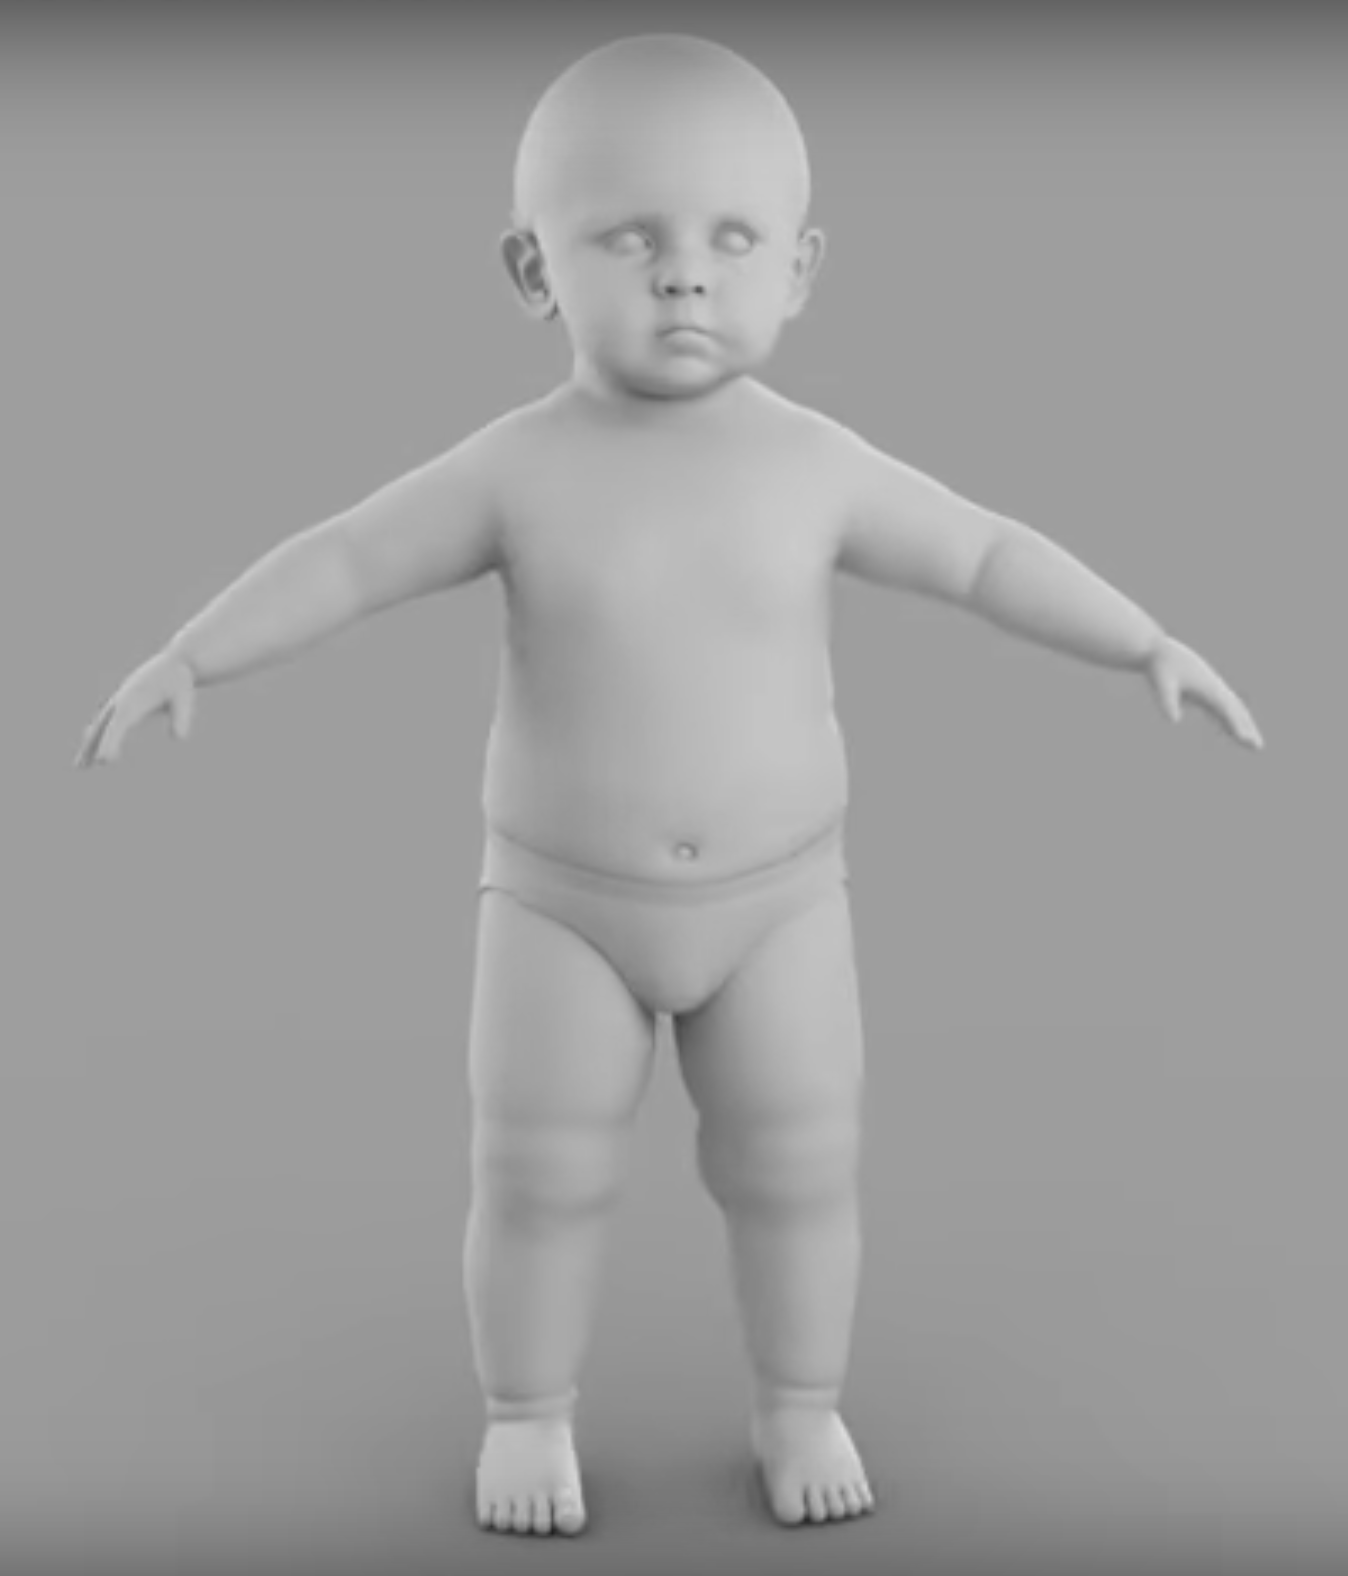
\includegraphics[width=7cm]{./bb1.png}
  \caption{\label{fig:bb1}
         Figures si necessaires, attention au copyright.}
\end{figure}


%-------------------------------------------------------------------------


\section{Conclusion}

%-------------------------------------------------------------------------

\bibliographystyle{eg-alpha}
\bibliography{mesreferences}
%va aller lire le fichier mesreferences.bib

\end{document}
